\section{Control de Formaciones en Sistemas Holonómicos}
\onecolumn
\subsection{Consenso con mantenimiento de formación}
Se parte del protocolo de Armel et al.~\cite{koulong2024distributed} y se modifica para agentes integradores, con $\nu_1=1$ y $\nu_2=\beta$:
\begin{align*}
    \dot{\mathbf{x}}_i &= \mathbf{u}_i \\[6pt]
    \mathbf{u}_i &=
    \underbrace{-\sum_{j \in \mathcal{N}_i} a_{ij}\big[(\mathbf{x}_i-\mathbf{r}_i)-(\mathbf{x}_j-\mathbf{r}_j)\big]}_{\text{\footnotesize Consenso entre vecinos}}
    \;\;
    \underbrace{-\,\beta\, b_i^0\big[(\mathbf{x}_i-\mathbf{r}_i)-\mathbf{x}_0\big]}_{\text{\footnotesize Atracción al ancla virtual}}
\end{align*}

\section{Control de Formaciones en Sistemas Holonómicos}
\onecolumn
\subsection{Consenso con mantenimiento de formación}
El desplazamiento $\mathbf{r}_i$ evita que el consenso colapse a los agentes en un punto y los sitúa en su lugar dentro de la formación. 

\begin{figure}[H]
    \centering
    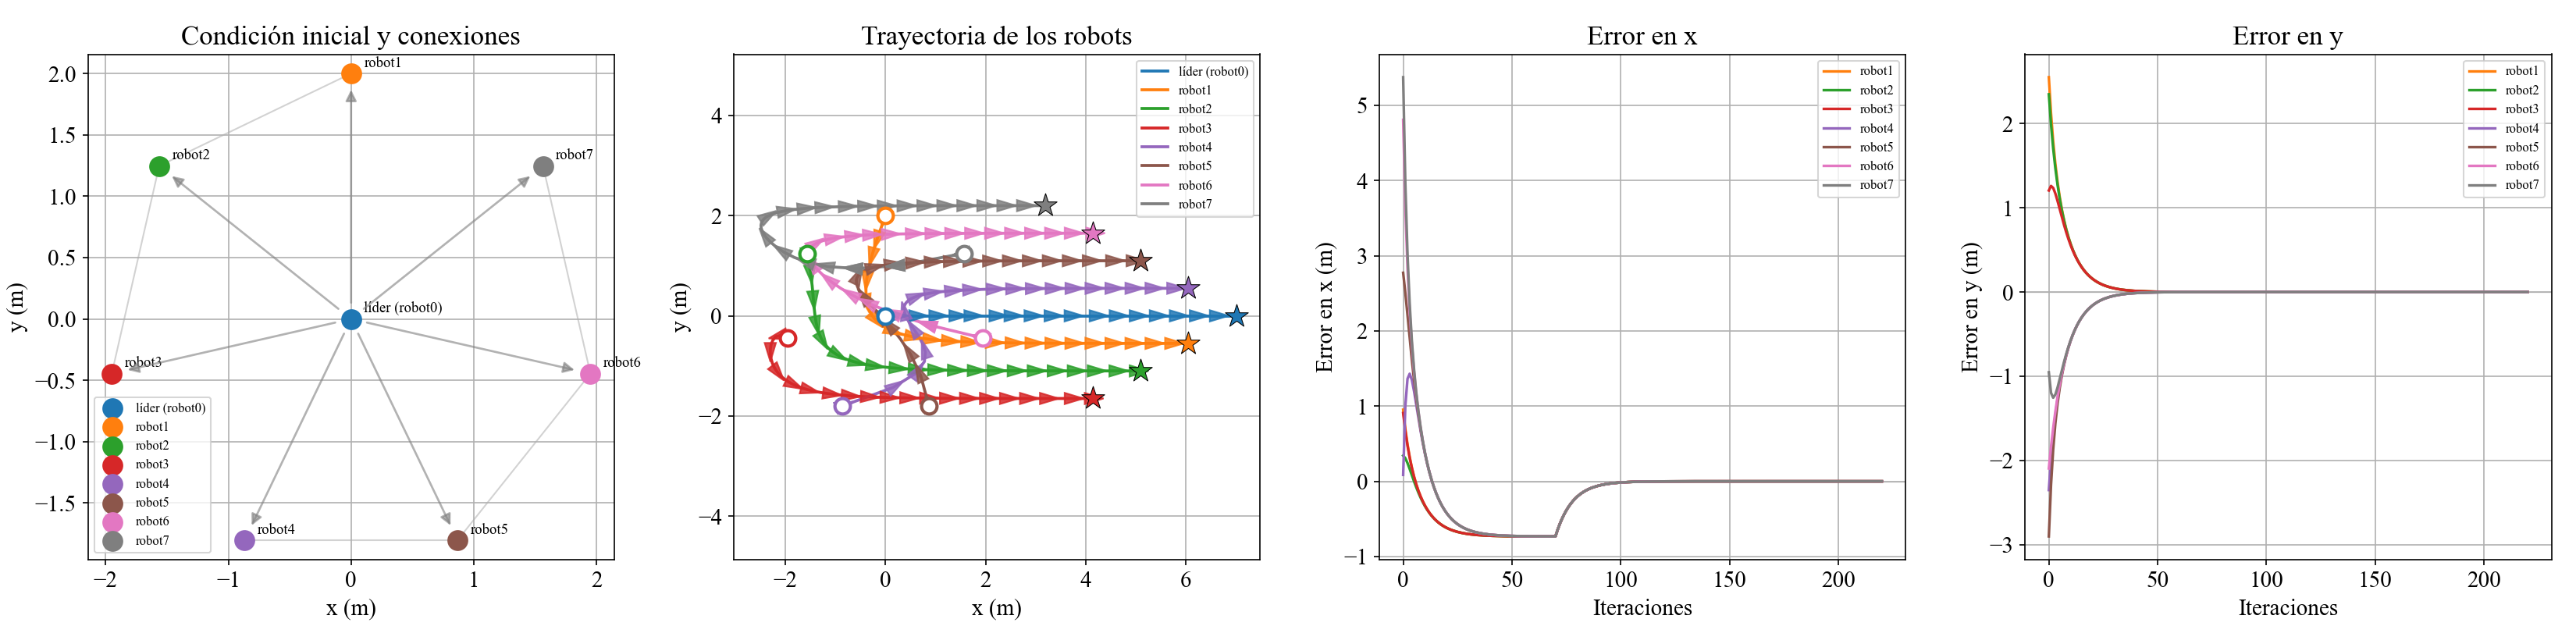
\includegraphics[width=\linewidth]{Pics/anclas_virtuales_resultado.png}
    \caption{Seguidores convergen hacia sus anclas virtuales}
    \label{fig:anclas_virtuales}
\end{figure}
